\documentclass[a4paper]{article}
    \usepackage{titlesec}
    \setcounter{secnumdepth}{4}
    \titleformat{\paragraph}
    {\normalfont\normalsize\bfseries}{\theparagraph}{1em}{}
    \titlespacing*{\paragraph}
    {0pt}{3.25ex plus 1ex minus .2ex}{1.5ex plus .2ex}

    \usepackage[T1]{fontenc}    %Codifica dei font
    \usepackage[utf8]{inputenc} %Lettere accentate da tastiera
    \usepackage[english]{babel} %Lingua del documento
    \usepackage{tabularx}       % extra features for tabular environment
    \usepackage{booktabs}
    \usepackage[table,xcdraw]{xcolor}
    \usepackage{siunitx}
    \usepackage{fancyvrb}
    \sisetup{output-decimal-marker={,}}
    \usepackage{graphicx} % takes care of graphic including machinery
    \usepackage[margin=0.75in,a4paper]{geometry} % decreases margins
    \usepackage[final]{hyperref} % adds hyper links inside the generated pdf file
    % \usepackage{minted}

    \newcommand{\polito }{\emph{Politecnico di Torino}}
    \newcommand{\oses}{\emph{Energy Management for IoT}}


    \begin{document}
    \title{
        Energy Management for IoT - Report Lab 02 \\[0.5cm]
        
\includegraphics[width=0.15\textwidth]{PoliLogo.png}%
    }
    \author{Flavia Caforio (s257750) - Samuele Yves Cerini (s256813)}
    \date{\today}
    \maketitle

    \tableofcontents

%   _____ _   _ _______ _____   ____  _____  _    _  _____ _______ _____ ____  _   _
%  |_   _| \ | |__   __|  __ \ / __ \|  __ \| |  | |/ ____|__   __|_   _/ __ \| \ | |
%    | | |  \| |  | |  | |__) | |  | | |  | | |  | | |       | |    | || |  | |  \| |
%    | | | . ` |  | |  |  _  /| |  | | |  | | |  | | |       | |    | || |  | | . ` |
%   _| |_| |\  |  | |  | | \ \| |__| | |__| | |__| | |____   | |   _| || |__| | |\  |
%  |_____|_| \_|  |_|  |_|  \_\\____/|_____/ \____/ \_____|  |_|  |_____\____/|_| \_|
%
\section{Introduction}
    The goal of this third and last laboratory is to model and simulate an IoT system by carefully evaluating its capabilities from a power consumption point of view. The final goal is to leverage the model (made using \emph{MATLAB/Simulink}) of the system and reach a satisfying level of power consumption, enough to reduce as much as possible the human intervention required to substitute the on-board battery. The system embeds four different ambient sensors, some memory and a control unit, a wireless transmission unit (using the \emph{ZigBee} protocol), a battery and a photovoltaic panel that will act as an energy scavenger, allowing us to recharge the battery and prolonging the lifespan of the overall system.
    
    In this report we will not discuss (as requested) the construction of the model or the configuration of the various components that are part of the system, but we will discuss directly the results obtained and the modifications done to the system itself in order to prolonge the system's battery life.

    This report is hence divided into 2 main parts:
    \begin{itemize}
        \item Workload definition to reduce the power consumption
        \item Modifications done to the system itself to increase its battery life
    \end{itemize}

%   _____           _     __
%  |  __ \         | |   /_ |
%  | |__) |_ _ _ __| |_   | |
%  |  ___/ _` | '__| __|  | |
%  | |  | (_| | |  | |_   | |
%  |_|   \__,_|_|   \__|  |_|
%
\section{Manipulating the system's workload}
    The goal of this first part of the laboratory is purely optimization-oriented: given the original model of the system, our goal is to maximize its battery life. By keeping the system as it is provided, without modifications, the only parameters we can modify are the different workloads submitted to the system, i.e. the load scheduling. The system, as mentioned before, is provided with four different sensors, a control unit and a transmission module. In order to optimize the battery life, we can modify how the different loads are activated, by choosing a good scheduling that minimizes the energy consumption.

    As a side note, we would like to inform the reader that all the following results have been taken with an activation period equal to 2 minutes. Different activation periods were initially proposed (like a period time of 10 minutes) but were finally withdrawn from the requests of the lab since such periods were sufficient to let the system run for an entire month, hence limiting our possibilities of analysis. Of course, some tests have been made with time periods equal to 10, 5 and 3 minutes, to observe the behavior of the system out of my curiosity, although the results have not been included in this report.

    \subsection{Sensors and Actuators characteristics}

    In table (\ref{tab:LoadSummary}) we reported the overall data available for every load attached to the system, retrieved directly from the related datasheets. Understanding what are the more demanding loads is crucial if we want to define a correct and balanced scheduling. 
    
    From the theory of DPM (Dynamic Power Management) we know for example that a "parallel" workload scheduling is not beneficial compared to "sequential" workload scheduling that spreads the load times along an entire period. In other words, it has been demonstrated multiple times that time limited bursts of high energy requests followed by long idle times are not beneficial as we may think.

    % Please add the following required packages to your document preamble:
    % \usepackage{booktabs}
    \begin{table}[]
        \centering
        \begin{tabular}{@{}llll@{}}
        \toprule
        Load                & Active Time (s) & Active Current (mA) & Sleep Current (mA) \\ \midrule
        Air Quality Sensor  & 30              & 48.2                & 0.002              \\
        Methane Sensor      & 30              & 18                  & 0.002              \\
        Temperature Sensor  & 6               & 3                   & 0.002              \\
        Microphone Sensor   & 12              & 0.15                & 0.002              \\
        ZigBee Transmission & 24              & 0.1                 & 0.001              \\
        Memory + Control    & 6               & 13                  & 0.002              \\ \bottomrule
        \end{tabular}
        \caption{Summary of the data linked to the loads attached to the system. The active time is fixed for each load and it depends on the requirements of the component.}
        \label{tab:LoadSummary}
    \end{table}

    \subsection{Sequential Workload}
        The first workload scheduling used is the one provided with the lab requirements: each one of the four sensors is activated sequentially, one after the other. The only constraints of the entire scheduling implies that we cannot process the data required before the completion of all the four sensors. At the same time, we cannot send the data (hence activating the transmitting module) prior the completion of the sensors load and the computation of the related data. 
        Thus, given these constraints, it is clear that the scheduling will have the last two loads related to the computation and the transmission of the retrieved data.

        As we mentioned before in the previous section, we expect this load to be quite good in terms of power consumption, due to its intrinsic wide scheduling (no small bursts of high energy requests are present).

        The provided scheduling is composed as follows:
        \begin{enumerate}
            \item Air Quality sensor;
            \item Methane sensor;
            \item Temperature sensor;
            \item Microphone sensor;
            \item Memory and Control;
            \item Transmission module;
        \end{enumerate}

        With the provided model and components, considering a period of activation equal to 2 minutes, the simulation of such workload scheduling resulted into a battery life of 588361 seconds, that corresponds to 6 days, 19 hours, 26 minutes. As we will see in the following sections, this load guaranteed the best result in terms of power consumption.

        The following image (\ref{fig:SeqLoadAndTOTPowerCurrent}) shows the workload scheduling as feeded to the model and simulated by \emph{Simulink}. In the bottom part of the graph we can see the load activation scheduling: we can appreciate the fact that the sequential approach spreads the load activation on the quasi entire period of activation (which corresponds to 2 minutes, i.e. 120 seconds). The top part of the graph shows, on the other hand, the current and the power consumption as required by the different load activations. From the graph, we can confirm that the Air Quality sensors has, for example, the highest current consumption among all the sensors ($48.2 mA$), which results in a power consumption of $48.2 mA \cdot 3.3V = 160mW$.

        In picture (\ref{fig:BattV-BattSoC-isDischargedV}) we reported the State of Charge and the voltage of the battery integrated in the system. As we can see, the battery is constantly discharging and the system is inevitably going to shut down itself. In some regions (that correspond to the regions where the solar panel harvests energy) the State of Charge stabilizes to a constant value or increases a little bit (still not significantly to avoid the complete discharge of the battery).

        In picture (\ref{fig:PVTotPower-Currents}) we can observe the trend of the current coming from the battery (\texttt{Battery Current}). This parameter if negative, indicates that the battery is being recharged. On the other hand, if the current has a positive sign, the current is absorbed from the battery to keep alive the entire system, hence discharging the battery. From this graph it is clear that more and more current is absorbed from the battery and that the graph area is greatly unbalanced towards the battery draining effect (a good system will have a graph more balanced that does not deviates towards more and more positive values, with an area beneath the graph which is equally balanced between negative zones and positive ones). From this same graph we can also observe the current provided by the photovoltaic module (\texttt{PV Current}) and the same current after the DCDC converters (\texttt{PV DCDC Current}) (that follow the module). We can observe the current attenuation due to the presence of the converters: adopting more expensive converters with higher efficiency can allow to reduce this attenuation and to obtain curves that are more and more close to themselves.

        \begin{figure}[htp]
            \centering
            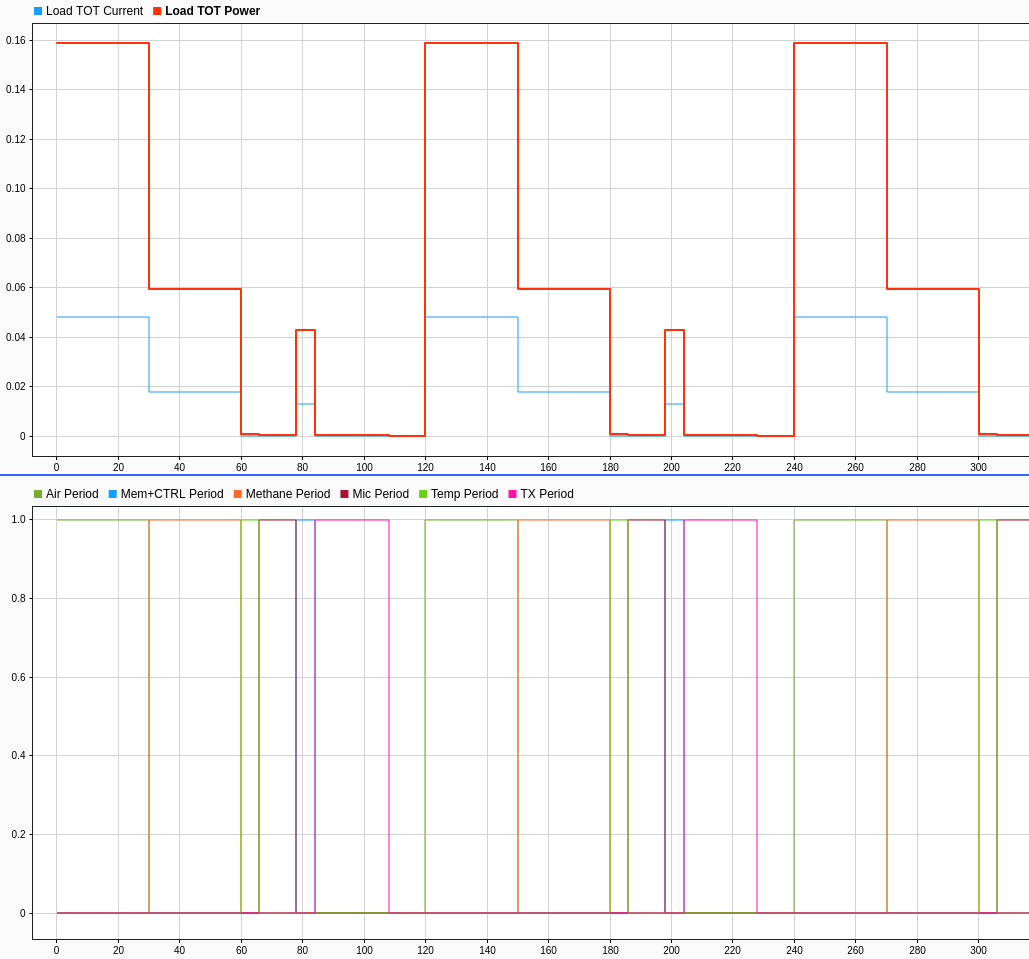
\includegraphics[width=1 \columnwidth]{./screenshots/SeqActiv/2Minutes/SeqLoadAndTOTPowerCurrent.png}
            \caption{
                    \label{fig:SeqLoadAndTOTPowerCurrent}
                    [Sequential Activation] Graph representing, in the bottom part, the sequential activation of all loads embedded in the system. In the top part, we can see the corresponding current and power consumption.
            }
        \end{figure}

        \begin{figure}[htp]
            \centering
            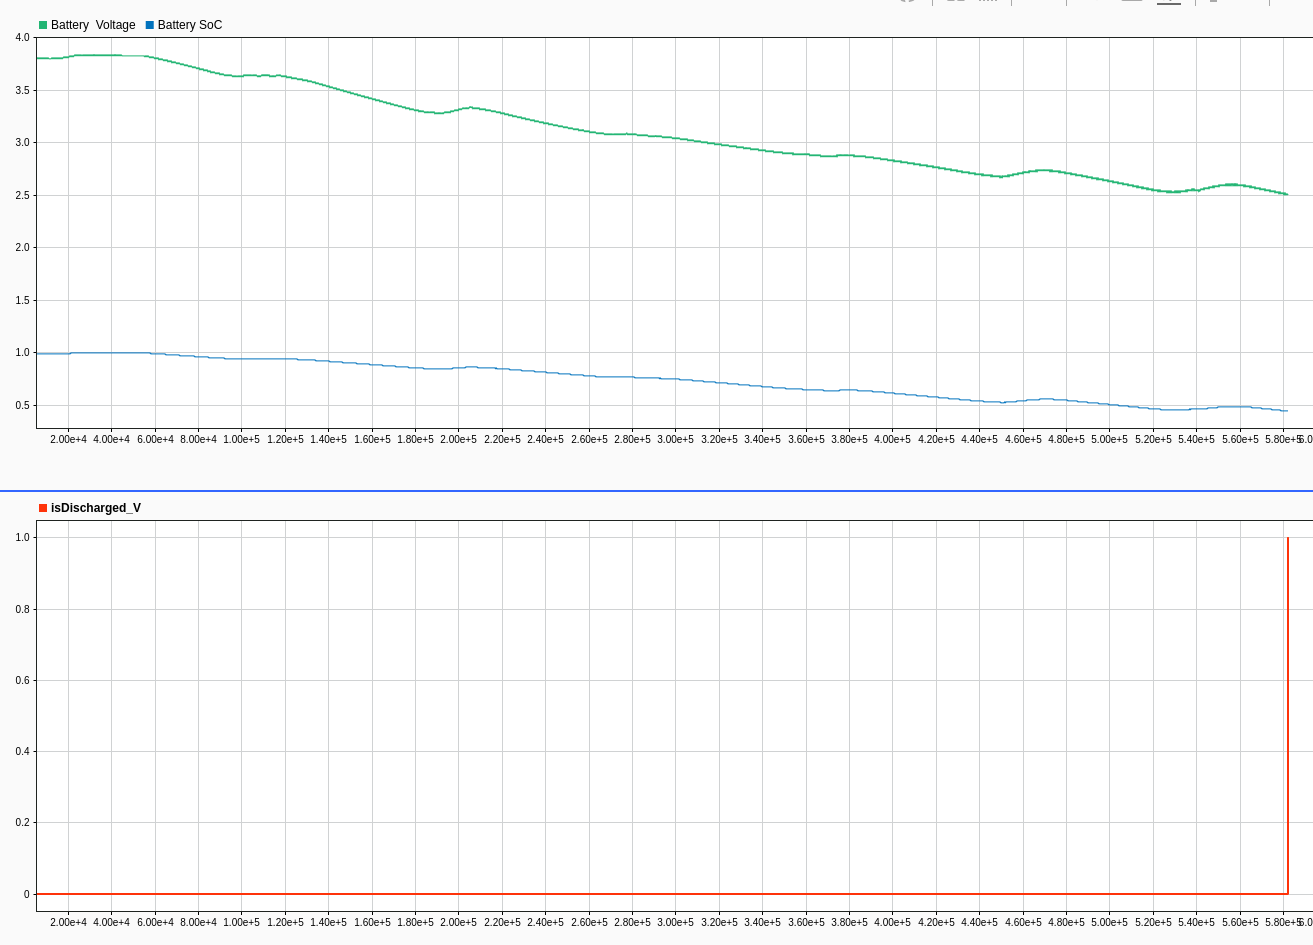
\includegraphics[width=0.8 \columnwidth]{./screenshots/SeqActiv/2Minutes/BattV-BattSoC-isDischargedV.png}
            \caption{
                    \label{fig:BattV-BattSoC-isDischargedV}
                    [Sequential Activation] Graphical representation of the State of Charge and the voltage of the battery. As we can see the battery is constantly discharged until the voltage reaches a threshold at which the battery is considered completely discharged (also indicated by the \texttt{isDischarged\_V} curve).
            }
        \end{figure}

        \begin{figure}[htp]
            \centering
            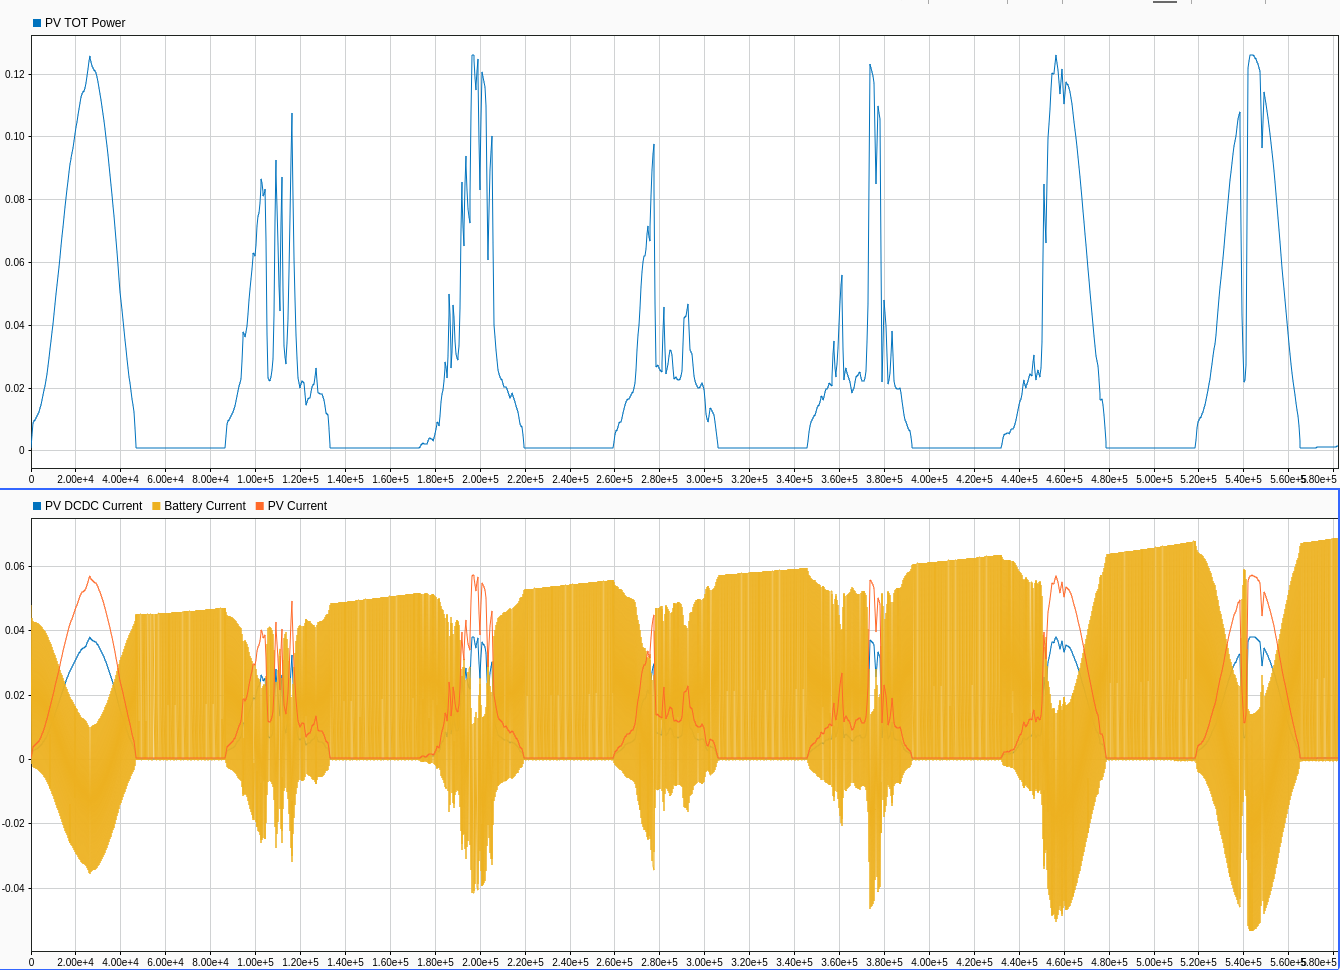
\includegraphics[width=1 \columnwidth]{./screenshots/SeqActiv/2Minutes/PVTotPower-Currents.png}
            \caption{
                    \label{fig:PVTotPower-Currents}
                    [Sequential Activation] Graph representing the battery current and the current provided by the photovoltaic panel (in the bottom section). In the top section we can appreciate the power produced by the solar panel.
            }
        \end{figure}

    \subsection{Parallel Workload}
        The second workload scheduling tested is the one that allows the parallel execution of loads, hence realizing a scheduling characterized by short bursts of current consumption and long idle times for each period (which remains also in this case set to 2 minutes). As mentioned before, we expected this workload scheduling to be the one less efficient in terms of energy consumption, leading to the poorest result in terms of battery life of the system.

        This hypothesis revealed to be true since we obtained a simulation that lasted up to 586229 seconds, equivalent to 6 days, 18 hours, 50 minutes and 29 seconds (and so approximately 36 minutes less than the Serial Scheduling tested in the previous section).

        From the first image (\ref{fig:ParLoadAndTOTPowerCurrent}) we can appreciate the load active time disposition, which follows as expected a parallel situation. On the top part of the graph we can, for example, observe that most of the power consumption happens in a short burst that lasts less than 40 seconds (even though the data transmission lasts up to 60 seconds, however its current consumption is minimal with respect to the one that happens before the 40 second threshold).

        From the second image (\ref{fig:ParBattV-BattSoC-isDischargedV}) we appreciate once again the State of Charge and the voltage of the battery. The bottom part indicates, once again, that the system is shut down due to the reaching of the lower threshold for the battery voltage: below that threshold the battery is considered to be completely discharged.

        Finally, the third figure (\ref{fig:ParLoadAndTOTPowerCurrent}) shows once again the current flowing to and from the battery, demonstrating the imbalance of the system once again.

        \begin{figure}[htp]
            \centering
            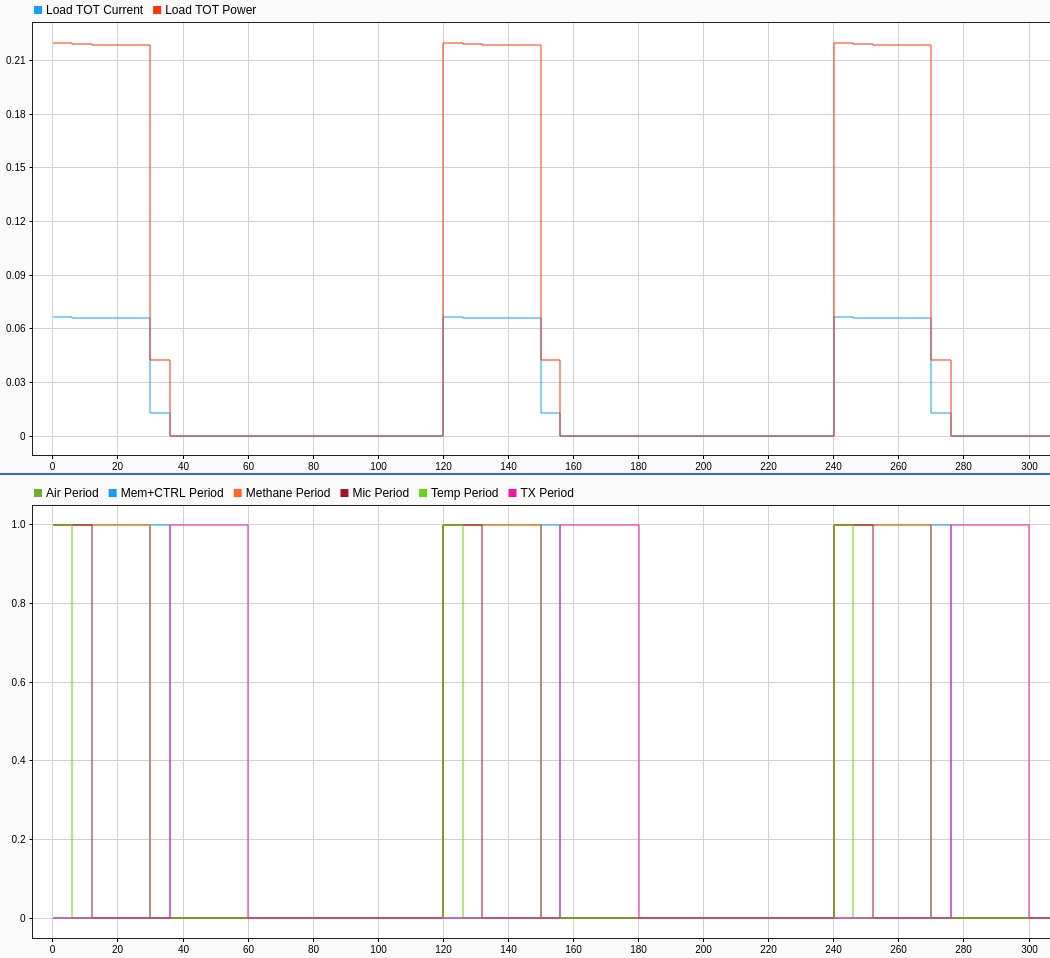
\includegraphics[width=1 \columnwidth]{./screenshots/ParActiv/2Minutes/ParLoadAndTOTPowerCurrent.png}
            \caption{
                    \label{fig:ParLoadAndTOTPowerCurrent}
                    [Parallel Activation] Graph representing, in the bottom part, the sequential activation of all loads embedded in the system. In the top part, we can see the corresponding current and power consumption.
            }
        \end{figure}

        \begin{figure}[htp]
            \centering
            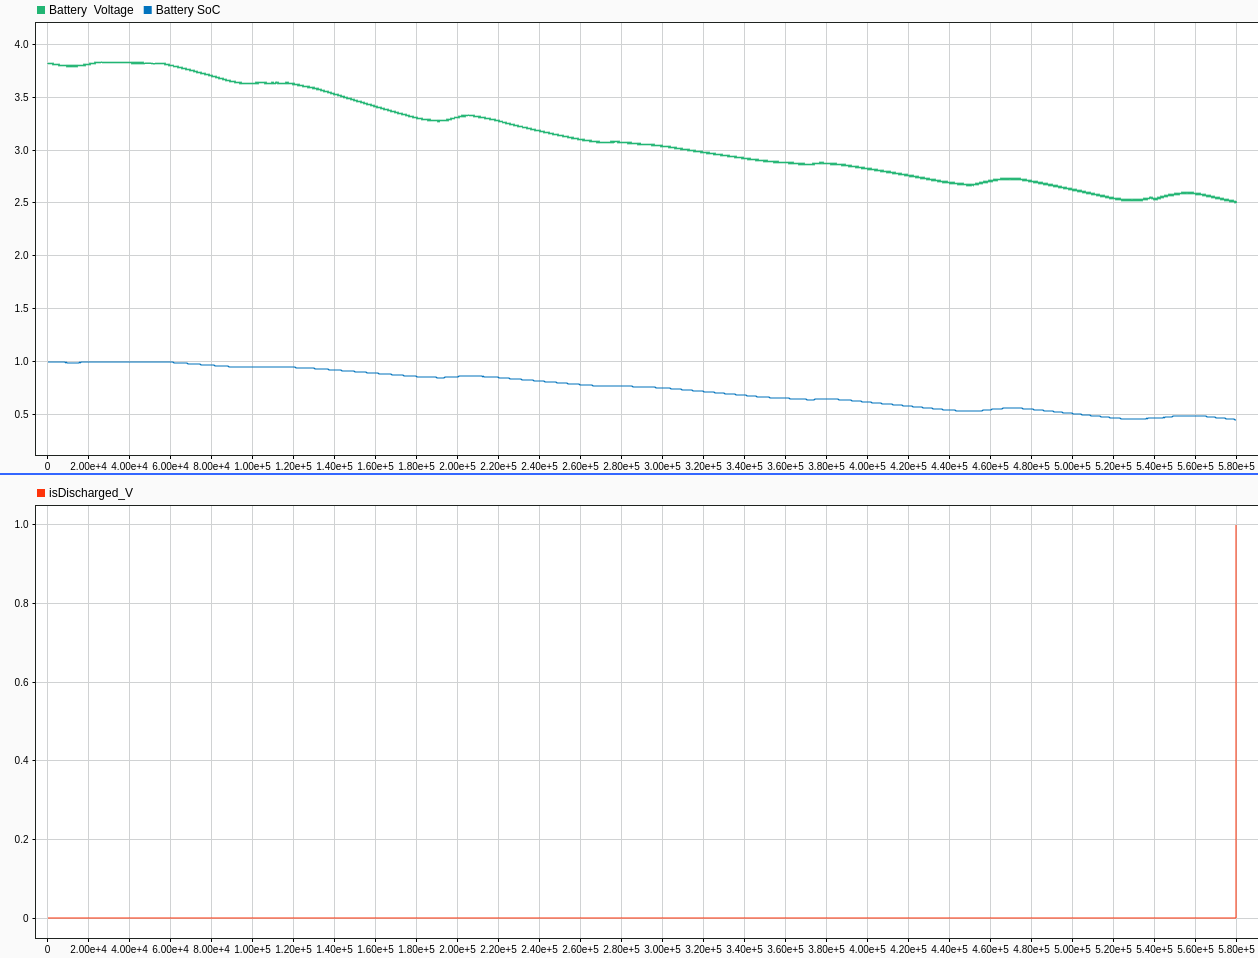
\includegraphics[width=0.8 \columnwidth]{./screenshots/ParActiv/2Minutes/BattV-BattSoC-isDischargedV.png}
            \caption{
                    \label{fig:ParBattV-BattSoC-isDischargedV}
                    [Parallel Activation] Graphical representation of the State of Charge and the voltage of the battery. As we can see the battery is constantly discharged until the voltage reaches a threshold at which the battery is considered completely discharged (also indicated by the \texttt{isDischarged\_V} curve).
            }
        \end{figure}

        \begin{figure}[htp]
            \centering
            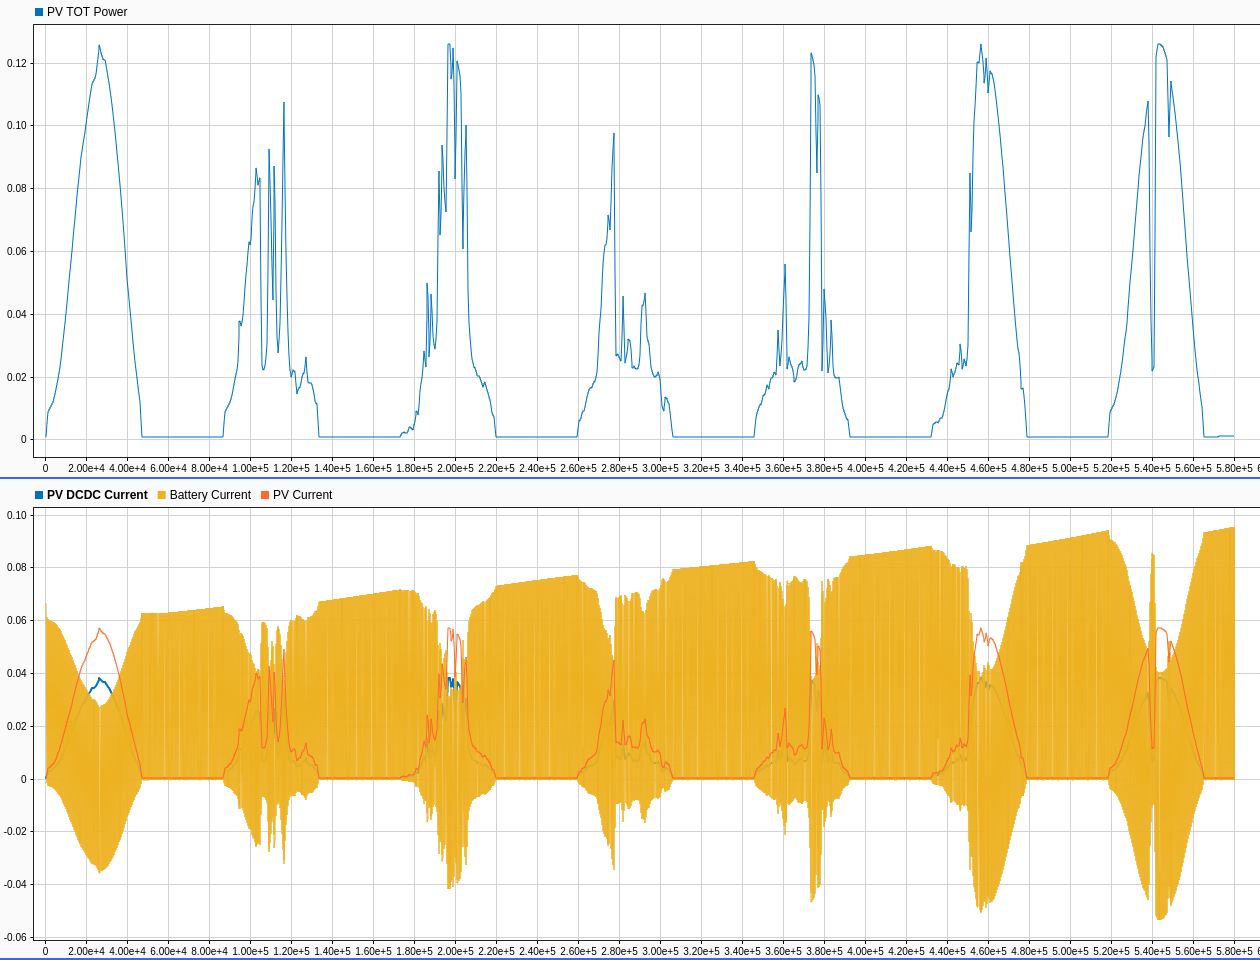
\includegraphics[width=1 \columnwidth]{./screenshots/ParActiv/2Minutes/PVTotPower-Currents.png}
            \caption{
                    \label{fig:ParPVTotPower-Currents}
                    [Parallel Activation] Graph representing the battery current and the current provided by the photovoltaic panel (in the bottom section). In the top section we can appreciate the power produced by the solar panel.
            }
        \end{figure}

    \subsection{Custom Solutions}
        I implemented two different workload schedulings as an attempt to reach higher lifetime of the system. As a general approach, I modified the provided Serial Scheduling, considered as a good starting point. The main idea is to better distribute the current consumption of the Serial Scheduling avoiding sharp peaks in energy consumption and having an overall "smoother" shape, following the shape of a gaussian distribution.
        Both schedulings simulated allowed to obtain very similar results: 
        \begin{itemize}
            \item Custom Scheduling \#1: 588360 seconds, equivalent to 6 days, 19 hours and 26 minutes (equivalent to the Serial Activation scheduling).
            \item Custom Scheduling \#2: 588291 seconds, equivalent to 6 days, 19 hours, 24 minutes and 51 seconds.
        \end{itemize}

        In the following image, we report the custom scheduling organization \#2 and the current consumption due to the load progression. If compared to the workload related to the Serial Activation, we can appreciate how high peaks of current consumption have been "smoothed" thanks to the different position of the loads activations. This allowed to obtain less noticeable current consumption swings.

        I decided to not report other graphs like the ones previously showed since the differences are not so marked and the two graphs will be quite comparable.

        \newpage

        In the following piece of code I report the construction of the two custom workloads:
        \begin{verbatim}
            % Custom #1: 588360 sec
            air_delay = 0;                      % first to execute
            methane_delay = air_time;           % second to execute
            temp_delay = air_time+mic_time;     % third to execute
            mic_delay = air_time;               % fourth to execute
            mc_delay = air_time + methane_time; % fifth to execute
            transmit_delay = mc_delay + mc_time;% sixth to execute
            
            % Custom #2: 588291 sec
            methane_delay = 0;                              % first to execute
            air_delay = methane_time;                       % second to execute
            temp_delay = methane_time-mic_time-temp_time;   % third to execute
            mic_delay = methane_time-mic_time;              % fourth to execute
            mc_delay = air_time + air_time;                 % fifth to execute
            transmit_delay = mc_delay + mc_time;            % sixth to execute
        \end{verbatim}

        \begin{figure}[htp]
            \centering
            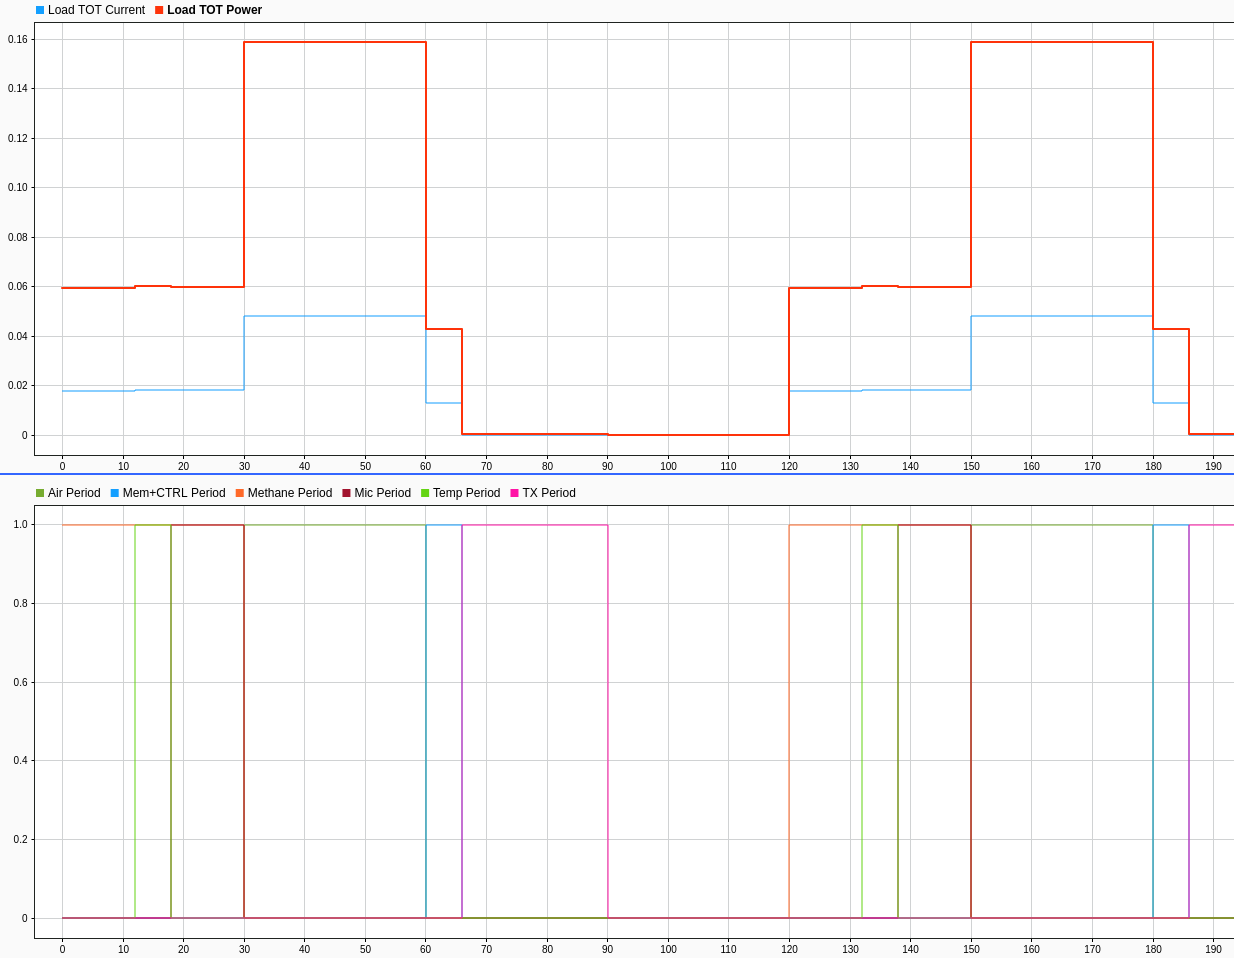
\includegraphics[width=1 \columnwidth]{./screenshots/SmartActiv/2Minutes/SmartLoadAndTOTPowerCurrent.png}
            \caption{
                    \label{fig:SmartLoadAndTOTPowerCurrent}
                    [Custom Activation \#2] Graph representing, in the bottom part, the sequential activation of all loads embedded in the system. In the top part, we can see the corresponding current and power consumption.
                    Please, notice how the total load current consumption has been "smoothed", allowing to have current swings less pronounced than the case obtained with the Sequential Activation (even more if we compare it to the Parallel Activation).
            }
        \end{figure}

        \subsubsection{Comments}
        Although the custom solutions seems to not provide evident benefices in terms of overall battery life of the system, we must take in mind the overall result "volatility" of the system and its dependency to the model construction and components definition. 
        These custom workloads have in fact have been simulated twice: the first time the coefficients of the converters were very similar to the actual ones but enough different to draw a quite different scenario in our system: with these latest coefficients that I've tried, all the workloads gained about 2 hours of lifetime. At the same time, these last coefficients resulted in a larger lifetime for the Serial Activation, overriding the previous best results I obtained with my custom workloads. That's why I was not able to apparently obtain a custom workload better than the one provided.

        Finally, I consider my workloads to be "less stressful" from a battery point of view with respect to the Serial Activation one: the reduction of the overall current swing probably allows to obtain less wear on the battery total life, finally allowing it to be recharged more times before its complete depletion.

%   _____           _     ___  
%  |  __ \         | |   |__ \ 
%  | |__) |_ _ _ __| |_     ) |
%  |  ___/ _` | '__| __|   / / 
%  | |  | (_| | |  | |_   / /_ 
%  |_|   \__,_|_|   \__| |____|
%                              
\section{System modifications and additions}
    
\end{document}